\chapter{角动量多重态、径向运动与振子阶梯}

\section{波函数的角依赖}

中心力场中的粒子具有一个径向坐标和两个角坐标。经典地，
\begin{equation}
\mathbf L=\mathbf r\times\mathbf p
\end{equation}
作为矢量守恒。其方向确定了轨道平面，尽管轨道不必是圆形的。

量子力学地，粒子由
\begin{equation}
\Psi=\Psi(r,\theta,\phi),
\end{equation}
描述，角动量涉及该波函数对角的依赖。

在二维中只有一个角动量分量，即绕垂直于平面的轴的旋转生成元：
\begin{equation}
L_z=-i\hbar\frac{\partial}{\partial\theta}.
\end{equation}
本征值为\(\hbar\ell\)的本征函数满足
\begin{equation}
-i\hbar\frac{\partial}{\partial\theta}\psi(r,\theta)
=\hbar\ell\,\psi(r,\theta).
\end{equation}
坐标\(r\)在该方程中是旁观者。其解具有形式
\begin{equation}
\psi(r,\theta)=\chi(r)e^{i\ell\theta}.
\end{equation}
对于普通的单值轨道波函数，在\(\theta\to\theta+2\pi\)之后回到同一点要求\(\ell\)为整数。径向因子\(\chi(r)\)可能影响能量，但不影响该角动量本征值。

三维类比将径向依赖与球面上的函数分离：
\begin{equation}
\Psi(r,\theta,\phi)=R(r)Y_{\ell m}(\theta,\phi).
\end{equation}
函数\(Y_{\ell m}\)是球谐函数。此处不需要其显式公式。旋转作用于角因子，而径向函数保持不变。

\section{有限角动量多重态}

角动量的分量满足
\begin{equation}
\begin{aligned}
[L_x,L_y]&=i\hbar L_z,\\
[L_y,L_z]&=i\hbar L_x,\\
[L_z,L_x]&=i\hbar L_y.
\end{aligned}
\end{equation}
选择\(L_z\)的本征态，
\begin{equation}
L_z|\ell,m\rangle=\hbar m\,|\ell,m\rangle,
\end{equation}
并定义
\begin{equation}
L_\pm=L_x\pm iL_y.
\end{equation}
对易关系
\begin{equation}
[L_z,L_\pm]=\pm\hbar L_\pm
\end{equation}
给出
\begin{align}
L_z\bigl(L_\pm|\ell,m\rangle\bigr)
&=\bigl(L_\pm L_z+[L_z,L_\pm]\bigr)|\ell,m\rangle \\
&=\hbar(m\pm1)L_\pm|\ell,m\rangle.
\end{align}
因此\(L_+\)将\(m\)升高一，而\(L_-\)将其降低一，除非所得矢量消失。

对于有限多重态，存在最高态和最低态：
\begin{equation}
L_+|\ell,\ell\rangle=0,
\qquad
L_-|\ell,-\ell\rangle=0.
\end{equation}
\(+z\)和\(-z\)方向通过旋转相联系，因此有限谱关于零对称。其值因此为
\begin{equation}
m=-\ell,-\ell+1,\ldots,\ell-1,\ell,
\end{equation}
而态数为
\begin{equation}
2\ell+1.
\end{equation}
由于相邻值相差一，端点可以是整数或半整数。普通轨道球谐函数实现整数情形；抽象角动量代数也允许半整数多重态。

\begin{classroomqa}
\lecturetimestamp{00:16:12}
\audiencequestion{角动量多重态能否包含无限多个态？}
\lecturerresponse{这种可能性可以考虑，但此处不需要。当态的其他特征保持不变时，角动量通常会提高能量，因此在讨论有限能量态时，无限角动量的态不相关。}
\end{classroomqa}

\section{\texorpdfstring{\(L^2\)}{L平方}}的共同值

测量角动量大小平方的算符是
\begin{equation}
L^2=L_x^2+L_y^2+L_z^2.
\end{equation}
阶梯算符的有序乘积为
\begin{align}
L_-L_+
&=(L_x-iL_y)(L_x+iL_y) \\
&=L_x^2+L_y^2+i[L_x,L_y] \\
&=L_x^2+L_y^2-\hbar L_z.
\end{align}
因此，
\begin{equation}
L^2=L_z^2+\hbar L_z+L_-L_+.
\end{equation}
将此恒等式应用于最高态。由于\(L_+|\ell,\ell\rangle=0\)，
\begin{align}
L^2|\ell,\ell\rangle
&=\left(L_z^2+\hbar L_z+L_-L_+\right)|\ell,\ell\rangle \\
&=\hbar^2\left(\ell^2+\ell\right)|\ell,\ell\rangle,
\end{align}
因此
\begin{equation}
L^2|\ell,\ell\rangle
=\hbar^2\ell(\ell+1)|\ell,\ell\rangle.
\end{equation}
平方大小不是\(\hbar^2\ell^2\)。额外项是角动量分量非对易性的结果。

同一个值属于多重态中的每一个态，而不仅是最高态。

\begin{classroomqa}
\lecturetimestamp{00:26:08}
\audiencequestion{证明其他态具有相同\(L^2\)值的练习究竟展示了什么？}
\lecturerresponse{证明\(L^2\)与角动量的每个分量对易，因此与\(L_-\)对易。然后将\(L^2\)通过\(L_-\)对易：如果最高态具有本征值\(\hbar^2\ell(\ell+1)\)，则下一个较低的态具有相同本征值。重复该论证将该值贯穿整个阶梯。}
\end{classroomqa}

确实，
\begin{equation}
[L^2,L_i]=0,
\qquad i=x,y,z,
\end{equation}
所以
\begin{equation}
[L^2,L_\pm]=0.
\end{equation}
例如，
\begin{align}
L^2\bigl(L_-|\ell,\ell\rangle\bigr)
&=L_-L^2|\ell,\ell\rangle \\
&=\hbar^2\ell(\ell+1)L_-|\ell,\ell\rangle.
\end{align}
继续向下给出
\begin{equation}
L^2|\ell,m\rangle
=\hbar^2\ell(\ell+1)|\ell,m\rangle
\end{equation}
对每个\(m=-\ell,\ldots,\ell\)。

相反的排序给出等价的因式分解：
\begin{align}
L_+L_-
&=(L_x+iL_y)(L_x-iL_y) \\
&=L_x^2+L_y^2-i[L_x,L_y] \\
&=L_x^2+L_y^2+\hbar L_z,
\end{align}
因此
\begin{equation}
L^2=L_z^2-\hbar L_z+L_+L_-.
\end{equation}

\begin{classroomqa}
\lecturetimestamp{00:32:05}
\audiencequestion{能否用\(L_+L_-\)将\(L_x^2+L_y^2\)按相反顺序因式分解？}
\lecturerresponse{可以。\(L_z\)项的符号会反转。按这种顺序，将恒等式作用于最低态，即被\(L_-\)湮灭的态，而不是作用于最高态。同样得到本征值\(\hbar^2\ell(\ell+1)\)。}
\end{classroomqa}

因此球谐函数满足
\begin{align}
L^2Y_{\ell m}
&=\hbar^2\ell(\ell+1)Y_{\ell m}, \\
L_zY_{\ell m}
&=\hbar m\,Y_{\ell m}.
\end{align}
对于每个轨道值\(\ell=0,1,2,\ldots\)，存在\(2\ell+1\)个由\(m=-\ell,\ldots,\ell\)标记的函数。

对于中心势，
\begin{equation}
[H,L_i]=0.
\end{equation}
一旦径向能量本征态和\(\ell\)固定，改变\(m\)并配合\(L_\pm\)不会改变能量。因此每个这样的径向本征态生成一个\(2\ell+1\)维磁多重态。

整数轨道阶梯如下所示。\footnote{该图根据讲座视频\(00{:}35{:}53\)处可见的多重态草图和算符恒等式重建。}

\begin{figure}[htbp]
\centering
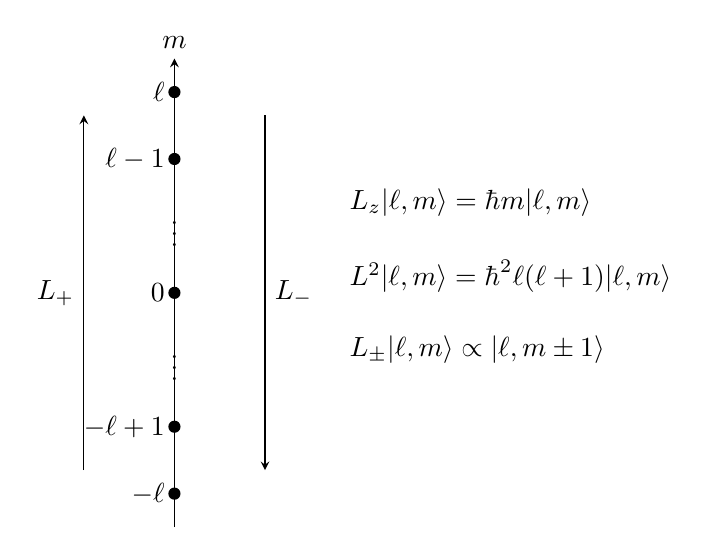
\begin{tikzpicture}[x=1cm,y=0.85cm,>=stealth]
\draw[->] (0,-3.5) -- (0,3.5) node[above] {$m$};

\fill (0,3) circle (2.2pt);
\fill (0,2) circle (2.2pt);
\fill (0,0) circle (2.2pt);
\fill (0,-2) circle (2.2pt);
\fill (0,-3) circle (2.2pt);

\node[left] at (0,3) {$\ell$};
\node[left] at (0,2) {$\ell-1$};
\node[left] at (0,0) {$0$};
\node[left] at (0,-2) {$-\ell+1$};
\node[left] at (0,-3) {$-\ell$};

\node at (0,1) {$\vdots$};
\node at (0,-1) {$\vdots$};

\draw[->] (-1.15,-2.65) -- (-1.15,2.65)
node[midway,left] {$L_+$};
\draw[->] (1.15,2.65) -- (1.15,-2.65)
node[midway,right] {$L_-$};

\node[anchor=west] at (2.1,1.35)
{$L_z|\ell,m\rangle=\hbar m|\ell,m\rangle$};
\node[anchor=west] at (2.1,0.25)
{$L^2|\ell,m\rangle=\hbar^2\ell(\ell+1)|\ell,m\rangle$};
\node[anchor=west] at (2.1,-0.85)
{$L_\pm|\ell,m\rangle\propto|\ell,m\pm1\rangle$};
\end{tikzpicture}
\caption{一个整数轨道角动量多重态。\(L_+\)和\(L_-\)将\(m\)改变一，而\(L^2\)在整个多重态中保持为\(\hbar^2\ell(\ell+1)\)。}
\lectureframe{00:35:53}
\end{figure}

\section{中心力问题}

考虑
\begin{equation}
H=\frac{\mathbf p^2}{2m}+V(r),
\end{equation}
其中\(V\)仅依赖于到原点的距离。旋转对称性意味着角动量守恒。经典地，\(\mathbf L\)具有固定的大小和方向，因此轨道保持在垂直于\(\mathbf L\)的平面内。轨道不必是圆形的，甚至不必是闭合的。

选择坐标使该经典轨道平面为\(xy\)平面，并将动量分解为径向和切向分量：
\begin{equation}
\mathbf p^2=p_r^2+p_\theta^2.
\end{equation}
由于角动量的大小为
\begin{equation}
L=r p_\theta,
\end{equation}
切向贡献可写为
\begin{equation}
p_\theta^2=\frac{L^2}{r^2}.
\end{equation}
哈密顿量变为
\begin{equation}
H=\frac{p_r^2}{2m}+\frac{L^2}{2mr^2}+V(r).
\end{equation}
对于固定的\(L\)，这是径向坐标中的一维问题，有效势为
\begin{equation}
V_{\mathrm{eff}}(r)=\frac{L^2}{2mr^2}+V(r).
\end{equation}
径向哈密顿量显示在下面的黑板上。\footnote{源帧：\texttt{\detokenize{lecture_03_frame_02.png}}，讲座视频在\(00{:}47{:}15\)。}

\begin{figure}[htbp]
\centering
\includegraphics[width=0.9\linewidth]{lecture_03_frame_02.png}
\caption{对于固定的经典角动量，径向哈密顿量包含径向动能、离心项\(L^2/(2mr^2)\)和中心势\(V(r)\)。}
\lectureframe{00:47:15}
\end{figure}

\(1/r^2\)项是离心势垒。当粒子接近原点时它升高，因此相应的力指向外。对于所讨论的类库仑吸引，具有\(L\neq0\)的轨迹会绕中心摆动而不是到达中心。当\(L=0\)时，势垒不存在。

对于吸引库仑势，
\begin{equation}
V(r)=-\frac{\kappa}{r},
\end{equation}
离心项在小\(r\)处占主导，而库仑项下降得更慢并在大\(r\)处占主导。对于\(L\neq0\)，它们的和有一个极小值。在极小值处的运动具有恒定半径，因此是圆形的。在极小值以上和逃逸阈值以下的束缚运动在最小半径和最大半径之间振荡；在库仑问题中，这些是椭圆轨道的径向振荡。

\section{约化径向方程}

在量子力学中，具有确定轨道角动量的态的角部分是球谐函数。将分离后的态写为
\begin{equation}
\Psi_{n_r\ell m}(r,\theta,\phi)
=\frac{u_{n_r\ell}(r)}{r}\,
Y_{\ell m}(\theta,\phi).
\end{equation}
角算符\(L^2\)具有本征值
\begin{equation}
L^2Y_{\ell m}
=\hbar^2\ell(\ell+1)Y_{\ell m}.
\end{equation}
对于固定的一对\(n_r,\ell\)，将\(u_{n_r\ell}(r)\)缩写为\(u(r)\)。留给约化径向函数的方程为
\begin{equation}
\begin{aligned}
&-\frac{\hbar^2}{2m}\frac{d^2u}{dr^2}
+\frac{\hbar^2\ell(\ell+1)}{2mr^2}u(r)\\
&\qquad+V(r)u(r)=E_{n_r\ell}\,u(r).
\end{aligned}
\end{equation}

\editorialnote{纯一维二阶导数方程使用约化径向函数\(u=rR\)。因此，讲座中展示的方程里的\(\psi(r)\)对应于\(u(r)\)，而\(\Psi=R(r)Y_{\ell m}\)中的普通径向因子是\(R=u/r\)。这种约定避免了将\(-i\hbar\,d/dr\)视为三维径向希尔伯特空间上独立的厄米径向动量算符。}

约化径向方程显示在下面的黑板上。\footnote{源帧：\texttt{\detokenize{lecture_03_frame_03.png}}，讲座视频在\(00{:}54{:}32\)。}

\begin{figure}[htbp]
\centering
\includegraphics[width=0.9\linewidth]{lecture_03_frame_03.png}
\caption{对于固定的\(\ell\)，约化径向波函数满足一个一维Schr\"odinger方程，其中包含一个正比于\(\ell(\ell+1)/r^2\)的离心项。}
\lectureframe{00:54:32}
\end{figure}

三维角结构已被压缩为参数\(\ell\)。磁量子数\(m\)不出现在径向方程中。

\begin{classroomqa}
\lecturetimestamp{00:55:34}
\audiencequestion{对于给定的\(\ell\)，\(2\ell+1\)个磁态是否具有相同的能量？}
\lecturerresponse{是的，前提是径向本征态也固定。对于每个选定的\(u_{n_r\ell}\)，所有值\(m=-\ell,\ldots,\ell\)具有相同的能量，因为\(m\)不进入径向方程。同一\(\ell\)下的不同径向本征态通常具有不同的能量。}
\end{classroomqa}

\begin{classroomqa}
\lecturetimestamp{00:56:03}
\audiencequestion{为什么\(L^2\)可以被\(\hbar^2\ell(\ell+1)\)替换，以及\(\ell\)与\(m\)的允许值有何关系？}
\lecturerresponse{数\(\ell\)标记一个角动量多重态，并且是该多重态中最大的\(m\)值。该多重态中的每个态都具有相同的\(L^2\)本征值\(\hbar^2\ell(\ell+1)\)，因此该本征值被代入径向方程。}
\end{classroomqa}

当前的论证不需要显式的特殊函数解。重要的是这些解是如何组织的。

\section{径向节点与能级}

对于固定的\(\ell\)，约化径向方程是一个普通的一维本征值问题。其束缚态按内部节点的数目排序。最低的径向态没有内部节点，下一个有一个，再下一个有两个。更多的节点意味着波函数变化更剧烈；变化更剧烈意味着动量更大，因而动能更大。

每个\(\ell\)值都定义了一个不同的径向算符，因为离心项随\(\ell\)变化。因此\(\ell=0,1,2,\ldots\)给出各自独立的径向能级序列。正的离心项随着角动量的增加将能级向上移动。在固定\(\ell\)下，每个径向本征值都带有一个维度为
\begin{equation}
2\ell+1.
\end{equation}
的磁多重态。\(\ell=0\)能级是单重态，\(\ell=1\)能级是三重态，\(\ell=2\)能级是五重态。这些是旋转对称性所保证的简并度；额外的对称性也可能使具有不同\(\ell\)值的态简并。

对于在大\(r\)处满足\(V(r)\to0\)的原子型势，逃逸阈值通常取为\(E=0\)。负能态构成离散的束缚谱。在\(E=0\)处及以上，遇到的是散射连续谱。这一陈述依赖于势的大\(r\)行为，不适用于具有禁闭作用的中心势。

\section{特殊的库仑简并}

精确的非相对论库仑势具有额外的能级对齐。最低的\(\ell=1\)径向态与第一激发\(\ell=0\)态具有相同的能量。下一个\(\ell=1\)态与第二激发\(\ell=0\)态对齐，而最低的\(\ell=2\)态也加入其中。这一模式在更高的径向和角动量序列中继续。

\begin{classroomqa}
\lecturetimestamp{01:09:57}
\audiencequestion{这种额外的库仑简并是否表明存在另一种对称性？}
\lecturerresponse{是的。它是精确库仑势的一种不寻常的额外对称性。势的微小变化会破坏这种对齐，其推导在此不予展开。}
\end{classroomqa}

由此得到的轨道壳层简并度为
\begin{equation}
1,\qquad 4,\qquad 9,\qquad 16,\qquad \ldots
\end{equation}
这是在计入电子自旋之前。

\begin{classroomqa}
\lecturetimestamp{01:11:46}
\audiencequestion{这种简并描述的是氢，还是仅描述理想的库仑问题？}
\lecturerresponse{氢以非常好的近似满足它，但并非精确满足。相对论修正和原子核的有限大小扰乱了理想的库仑模式。}
\end{classroomqa}

点核产生精确的\(1/r\)势。电荷分布在微小体积内的核，当电子穿透该体积时会产生略微不同的势，而即使这种微小的偏离也会解除部分特殊简并。

自旋也被省略了。计入两个电子自旋态后，壳层计数加倍为
\begin{equation}
2,\qquad 8,\qquad 18,\qquad 32,\qquad \ldots
\end{equation}
这是在更完整的原子处理所分辨出的进一步分裂之前。

\section{重访笛卡尔方程}

径向问题所由出发的方程是三维定态Schr\"odinger方程
\begin{equation}
\begin{aligned}
-\frac{\hbar^2}{2m}\nabla^2\Psi+V(r)\Psi&=E\Psi,\\
\nabla^2&=\frac{\partial^2}{\partial x^2}
+\frac{\partial^2}{\partial y^2}
+\frac{\partial^2}{\partial z^2},\\
r&=\sqrt{x^2+y^2+z^2}.
\end{aligned}
\end{equation}
过渡到径向坐标和角坐标，并选取\(L^2\)的一个本征态。将\(L^2\)替换为\(\hbar^2\ell(\ell+1)\)，就把偏微分方程约化为上面的常微分径向方程。

\begin{classroomqa}
\lecturetimestamp{01:16:42}
\audiencequestion{能否利用对理想库仑谱的偏离来确定原子核的大小？}
\lecturerresponse{不能通过这种简单的比较。其他修正要大得多，必须首先加以考虑。这里提到核大小，是因为它给出了一个偏离点库仑势的直接例子。}
\end{classroomqa}

\begin{classroomqa}
\lecturetimestamp{01:17:09}
\audiencequestion{经典角动量项与量子角动量项之间的主要区别是什么？}
\lecturerresponse{经典地，\(L^2\)是一个守恒矢量大小的普通平方。在量子轨道多重态中，其本征值是\(\hbar^2\ell(\ell+1)\)，而不简单地是\(\hbar^2\ell^2\)。额外的项来自角动量分量之间的不对易性。}
\end{classroomqa}

\begin{classroomqa}
\lecturetimestamp{01:17:58}
\audiencequestion{束缚态波函数具有紧支集吗？}
\lecturerresponse{不。它们会延伸到离中心任意远的地方。对于所讨论的原子束缚态，它们在远距离处按指数衰减，因此概率变得可以忽略，但在任何有限半径之外并不为零。}
\end{classroomqa}

\begin{classroomqa}
\lecturetimestamp{01:18:48}
\audiencequestion{当\(\ell=0\)移除离心势阱时，稳定点会变成什么？}
\lecturerresponse{不再存在由离心势垒与吸引之间的竞争所产生的最小值。在点库仑理想化中，经典运动趋向奇异的中心。在量子力学中，最低态不可能同时具有位于中心的完全确定的位置和零动量，因此最低波函数具有有限的空间延展。}
\end{classroomqa}

\editorialnote{对于规则的中心势，经典零角动量轨道可以穿过原点继续运动。对于理想的点库仑势，\(r=0\)反而是碰撞奇点，经典轨道的延续需要额外的规定。}

经典约化将单一轨道置于一个平面内，但这一步骤不能以同样的方式应用于量子波函数。量子轨道态充满三维空间。完整的角动量算符是\(L^2=L_x^2+L_y^2+L_z^2\)，其特征值保留三维结果\(\hbar^2\ell(\ell+1)\)。

\begin{classroomqa}
\lecturetimestamp{01:21:30}
\audiencequestion{在经典轨道被置于平面内之后，量子问题如何仍能保持三维？}
\lecturerresponse{只有经典轨道通过选择垂直于其守恒角动量矢量的坐标而被置于固定平面内。量子波函数占据三维空间。其他角动量分量通过\(L^2\)仍然存在，这就是为什么径向方程包含\(\ell(\ell+1)\)，而不仅仅是一个分量的平方。}
\end{classroomqa}

\begin{classroomqa}
\lecturetimestamp{01:22:54}
\audiencequestion{是否每个量子问题都允许有升算符和降算符？}
\lecturerresponse{不。它们出现在异常有利的情形中。角动量就是这样一个情形，谐振子则是另一个。谐振子的情形特别有用，因为稳定平衡附近的运动常常近似为简谐的，包括有效势最小值附近的小径向振荡。}
\end{classroomqa}

原子问题在此暂时搁置，谐振子成为下一个由阶梯算符确定谱的例子。

\section{小振动与谐振子}

在稳定平衡附近，足够小的位移常常产生简谐运动。非零角动量的有效径向势提供了一个例子：在其势阱底部附近的径向运动近似为简谐的。

考虑一个单位质量的一维振子。设\(x\)为偏离平衡的位移，并将弹簧常数写为\(k=\omega^2\)。经典哈密顿量为
\begin{equation}
H=\frac{p^2}{2}+\frac{\omega^2x^2}{2}.
\end{equation}
哈密顿方程给出
\begin{equation}
\dot{x}=\frac{\partial H}{\partial p}=p,
\qquad
\dot{p}=-\frac{\partial H}{\partial x}=-\omega^2x,
\end{equation}
因此
\begin{equation}
\ddot{x}=-\omega^2x.
\end{equation}
于是\(\omega\)是经典振荡频率。

\section{因式分解与零点能}

在量子力学中，
\begin{equation}
[x,p]=i\hbar.
\end{equation}
哈密顿量是平方之和，这提示因式分解
\begin{align}
\frac{1}{2}(p+i\omega x)(p-i\omega x)
&=\frac{1}{2}\left(p^2+\omega^2x^2+i\omega[x,p]\right) \\
&=\frac{1}{2}\left(p^2+\omega^2x^2-\hbar\omega\right).
\end{align}
因此
\begin{equation}
H=\frac{1}{2}(p+i\omega x)(p-i\omega x)
+\frac{1}{2}\hbar\omega.
\end{equation}
附加项\(\hbar\omega/2\)是零点能。

经典上最低能量会出现在\(x=p=0\)处。在量子力学中，没有任何态能够同时将位置和动量都精确固定在零。此外，两项\(p^2/2\)和\(\omega^2x^2/2\)都是正的，不能相互抵消。因此非零的基态能量是不可避免的。

对于阶梯计算，可以暂时将共同的附加常数搁置一旁，最后再恢复。

\begin{classroomqa}
\lecturetimestamp{01:36:10}
\audiencequestion{零点能项的正号是否还告诉我们更多信息？}
\lecturerresponse{振子哈密顿量是一个正算符：它是正平方之和，因此其能量不可能为负。}
\end{classroomqa}

\section{振子阶梯}

引入无量纲算符\footnote{在\(01{:}37\)--\(01{:}42\)附近，计算采用\(\hbar=1\)。在这些归一化定义中恢复\(\hbar\)因子，是为了使\(A_\pm\)无量纲，且其对易子为1。}
\begin{equation}
A_+=\frac{p+i\omega x}{\sqrt{2\hbar\omega}},
\qquad
A_-=\frac{p-i\omega x}{\sqrt{2\hbar\omega}}.
\end{equation}
它们互为厄米共轭：
\begin{equation}
A_+^\dagger=A_-.
\end{equation}
它们的对易子为
\begin{align}
[A_-,A_+]
&=\frac{1}{2\hbar\omega}
\left([p,i\omega x]+[-i\omega x,p]\right) \\
&=1.
\end{align}


定义
\begin{equation}
N=A_+A_-.
\end{equation}
则哈密顿量为
\begin{equation}
H=\hbar\omega\left(N+\frac{1}{2}\right).
\end{equation}
因此，求能量谱归结为求\(N\)的本征值。

假设
\begin{equation}
N|n\rangle=n|n\rangle.
\end{equation}
与\(N\)的对易子是\footnote{在\(01{:}45{:}37\)--\(01{:}48{:}10\)处的中间步骤直接由所述关系\(N=A_+A_-\)和\([A_-,A_+]=1\)重构。}
\begin{align}
[N,A_+]
&=A_+[A_-,A_+]=A_+, \\
[N,A_-]
&=[A_+,A_-]A_-=-A_-.
\end{align}
由此可得
\begin{align}
N\bigl(A_+|n\rangle\bigr)
&=(n+1)A_+|n\rangle, \\
N\bigl(A_-|n\rangle\bigr)
&=(n-1)A_-|n\rangle.
\end{align}
因此，只要所得矢量非零，\(A_+\)就把\(N\)的一个本征值升高1，而\(A_-\)把它降低1。

算符\(N\)是非负的：
\begin{equation}
\langle\psi|N|\psi\rangle
=\langle\psi|A_+A_-|\psi\rangle
=\|A_-|\psi\rangle\|^2
\geq0.
\end{equation}
因此，降低过程不能继续进入负本征值。在一个底态\(|b\rangle\)处，它必须终止：
\begin{equation}
A_-|b\rangle=0.
\end{equation}

对于归一化本征态，阶梯中的系数由它们的范数确定：
\begin{align}
\|A_-|n\rangle\|^2
&=\langle n|A_+A_-|n\rangle=n, \\
\|A_+|n\rangle\|^2
&=\langle n|A_-A_+|n\rangle=n+1.
\end{align}
因此可以选取相位使得
\begin{equation}
A_-|n\rangle=\sqrt{n}\,|n-1\rangle,
\qquad
A_+|n\rangle=\sqrt{n+1}\,|n+1\rangle.
\end{equation}

\begin{classroomqa}
\lecturetimestamp{01:52:42}
\audiencequestion{如果\(A_-\)降低一个态，而\(A_+\)把它升回去，那么\(A_+A_-\)如何产生本征值\(n\)？}
\lecturerresponse{阶梯作用包含归一化因子。先用\(A_-\)作用贡献\(\sqrt n\)，再用\(A_+\)作用于所得态又贡献一个\(\sqrt n\)。它们的乘积是\(n\)。}
\end{classroomqa}

确实，
\begin{equation}
A_+A_-|n\rangle
=\sqrt n\,A_+|n-1\rangle
=n|n\rangle.
\end{equation}

\begin{classroomqa}
\lecturetimestamp{01:55:52}
\audiencequestion{\(N\)的最低本征值必须是零吗，还是可以是正的？}
\lecturerresponse{它必须是零，并且\(N\)的谱由非负整数组成。关于端点情形的证明尚未给出。}
\end{classroomqa}

\editorialnote{设\(|b\rangle\)是一个最低态。由于降低必须终止，\(A_-|b\rangle=0\)。由此立即得到\(N|b\rangle=A_+A_-|b\rangle=0\)，所以\(N\)的最低本征值是零。}

从这个最低态出发并作用\(A_+\)，得到
\begin{equation}
n=0,1,2,\ldots.
\end{equation}
恢复加性零点项后，振子能量为
\begin{equation}
E_n=\hbar\omega\left(n+\frac{1}{2}\right),
\qquad n=0,1,2,\ldots.
\end{equation}

振子代数将进一步发展，并用于求解其他量子问题。
